%% abtex2-modelo-trabalho-academico.tex, v-1.9.2 laurocesar
%% Copyright 2012-2014 by abnTeX2 group at http://abntex2.googlecode.com/ 
%%
%% This work may be distributed and/or modified under the
%% conditions of the LaTeX Project Public License, either version 1.3
%% of this license or (at your option) any later version.
%% The latest version of this license is in
%%   http://www.latex-project.org/lppl.txt
%% and version 1.3 or later is part of all distributions of LaTeX
%% version 2005/12/01 or later.
%%
%% This work has the LPPL maintenance status `maintained'.
%% 
%% The Current Maintainer of this work is the abnTeX2 team, led
%% by Lauro César Araujo. Further information are available on 
%% http://abntex2.googlecode.com/
%%
%% This work consists of the files abntex2-modelo-trabalho-academico.tex,
%% abntex2-modelo-include-comandos and abntex2-modelo-references.bib
%%

% ------------------------------------------------------------------------
% ------------------------------------------------------------------------
% abnTeX2: Modelo de Trabalho Academico (tese de doutorado, dissertacao de
% mestrado e trabalhos monograficos em geral) em conformidade com 
% ABNT NBR 14724:2011: Informacao e documentacao - Trabalhos academicos -
% Apresentacao
% ------------------------------------------------------------------------
% ------------------------------------------------------------------------

\documentclass[
	% -- opções da classe memoir --
	12pt,				% tamanho da fonte
	openright,			% capítulos começam em pág ímpar (insere página vazia caso preciso)
	twoside,			% para impressão em verso e anverso. Oposto a oneside
	a4paper,			% tamanho do papel. 
	% -- opções da classe abntex2 --
	%chapter=TITLE,		% títulos de capítulos convertidos em letras maiúsculas
	%section=TITLE,		% títulos de seções convertidos em letras maiúsculas
	%subsection=TITLE,	% títulos de subseções convertidos em letras maiúsculas
	%subsubsection=TITLE,% títulos de subsubseções convertidos em letras maiúsculas
	% -- opções do pacote babel --
	english,			% idioma adicional para hifenização
	french,				% idioma adicional para hifenização
	spanish,			% idioma adicional para hifenização
	brazil				% o último idioma é o principal do documento
	]{abntex2}

% ---
% Pacotes básicos 
% ---
\usepackage{lmodern}			% Usa a fonte Latin Modern			
\usepackage[T1]{fontenc}		% Selecao de codigos de fonte.
\usepackage[utf8]{inputenc}		% Codificacao do documento (conversão automática dos acentos)
\usepackage{lastpage}			% Usado pela Ficha catalográfica
\usepackage{indentfirst}		% Indenta o primeiro parágrafo de cada seção.
\usepackage{color}				% Controle das cores
\usepackage{graphicx}			% Inclusão de gráficos
\usepackage{microtype} 			% para melhorias de justificação
% ---

% ---
% Pacotes adicionais, usados apenas no âmbito do Modelo Canônico do abnteX2
% ---
\usepackage{pdfpages}
\usepackage{algorithm}				% para geração de dummy text
\usepackage{algpseudocode}				% para geração de dummy text
% ---

% ---
% Pacotes de citações
% ---
\usepackage[brazilian,hyperpageref]{backref}	 % Paginas com as citações na bibl
\usepackage[alf]{abntex2cite}	% Citações padrão ABNT

% --- 
% CONFIGURAÇÕES DE PACOTES
% --- 

% ---
% Configurações do pacote backref
% Usado sem a opção hyperpageref de backref
\renewcommand{\backrefpagesname}{Citado na(s) página(s):~}
% Texto padrão antes do número das páginas
\renewcommand{\backref}{}
% Define os textos da citação
\renewcommand*{\backrefalt}[4]{
	\ifcase #1 %
		Nenhuma citação no texto.%
	\or
		Citado na página #2.%
	\else
		Citado #1 vezes nas páginas #2.%
	\fi}%
% ---

% ---
% Informações de dados para CAPA e FOLHA DE ROSTO
% ---
\titulo{Modelo Canônico de\\ Trabalho Acadêmico com \abnTeX}
\autor{Equipe \abnTeX}
\local{Brasil}
\data{2014, v-1.9.2}
\orientador{Lauro César Araujo}
\coorientador{Equipe \abnTeX}
\instituicao{%
  Universidade do Brasil -- UBr
  \par
  Faculdade de Arquitetura da Informação
  \par
  Programa de Pós-Graduação}
\tipotrabalho{Tese (Doutorado)}
% O preambulo deve conter o tipo do trabalho, o objetivo, 
% o nome da instituição e a área de concentração 
\preambulo{Modelo canônico de trabalho monográfico acadêmico em conformidade com
as normas ABNT apresentado à comunidade de usuários \LaTeX.}
% ---


% ---
% Configurações de aparência do PDF final

% alterando o aspecto da cor azul
\definecolor{blue}{RGB}{41,5,195}

% informações do PDF
\makeatletter
\hypersetup{
     	%pagebackref=true,
		pdftitle={\@title}, 
		pdfauthor={\@author},
    	pdfsubject={\imprimirpreambulo},
	    pdfcreator={LaTeX with abnTeX2},
		pdfkeywords={abnt}{latex}{abntex}{abntex2}{trabalho acadêmico}, 
		colorlinks=true,       		% false: boxed links; true: colored links
    	linkcolor=blue,          	% color of internal links
    	citecolor=blue,        		% color of links to bibliography
    	filecolor=magenta,      		% color of file links
		urlcolor=blue,
		bookmarksdepth=4
}
\makeatother
% --- 

% --- 
% Espaçamentos entre linhas e parágrafos 
% --- 

% O tamanho do parágrafo é dado por:
\setlength{\parindent}{1.3cm}

% Controle do espaçamento entre um parágrafo e outro:
\setlength{\parskip}{0.2cm}  % tente também \onelineskip

% ---
% compila o indice
% ---
\makeindex
% ---

% ----
% Início do documento
% ----
\begin{document}

% Retira espaço extra obsoleto entre as frases.
\frenchspacing 

% ----------------------------------------------------------
% ELEMENTOS PRÉ-TEXTUAIS
% ----------------------------------------------------------
% ---
% Capa
% ---
\imprimircapa
% ---

% ---
% Folha de rosto
% (o * indica que haverá a ficha bibliográfica)
% ---
\imprimirfolhaderosto*
% ---

% ---
% Inserir a ficha bibliografica
% ---
% http://ficha.bu.ufsc.br/
\begin{fichacatalografica}
	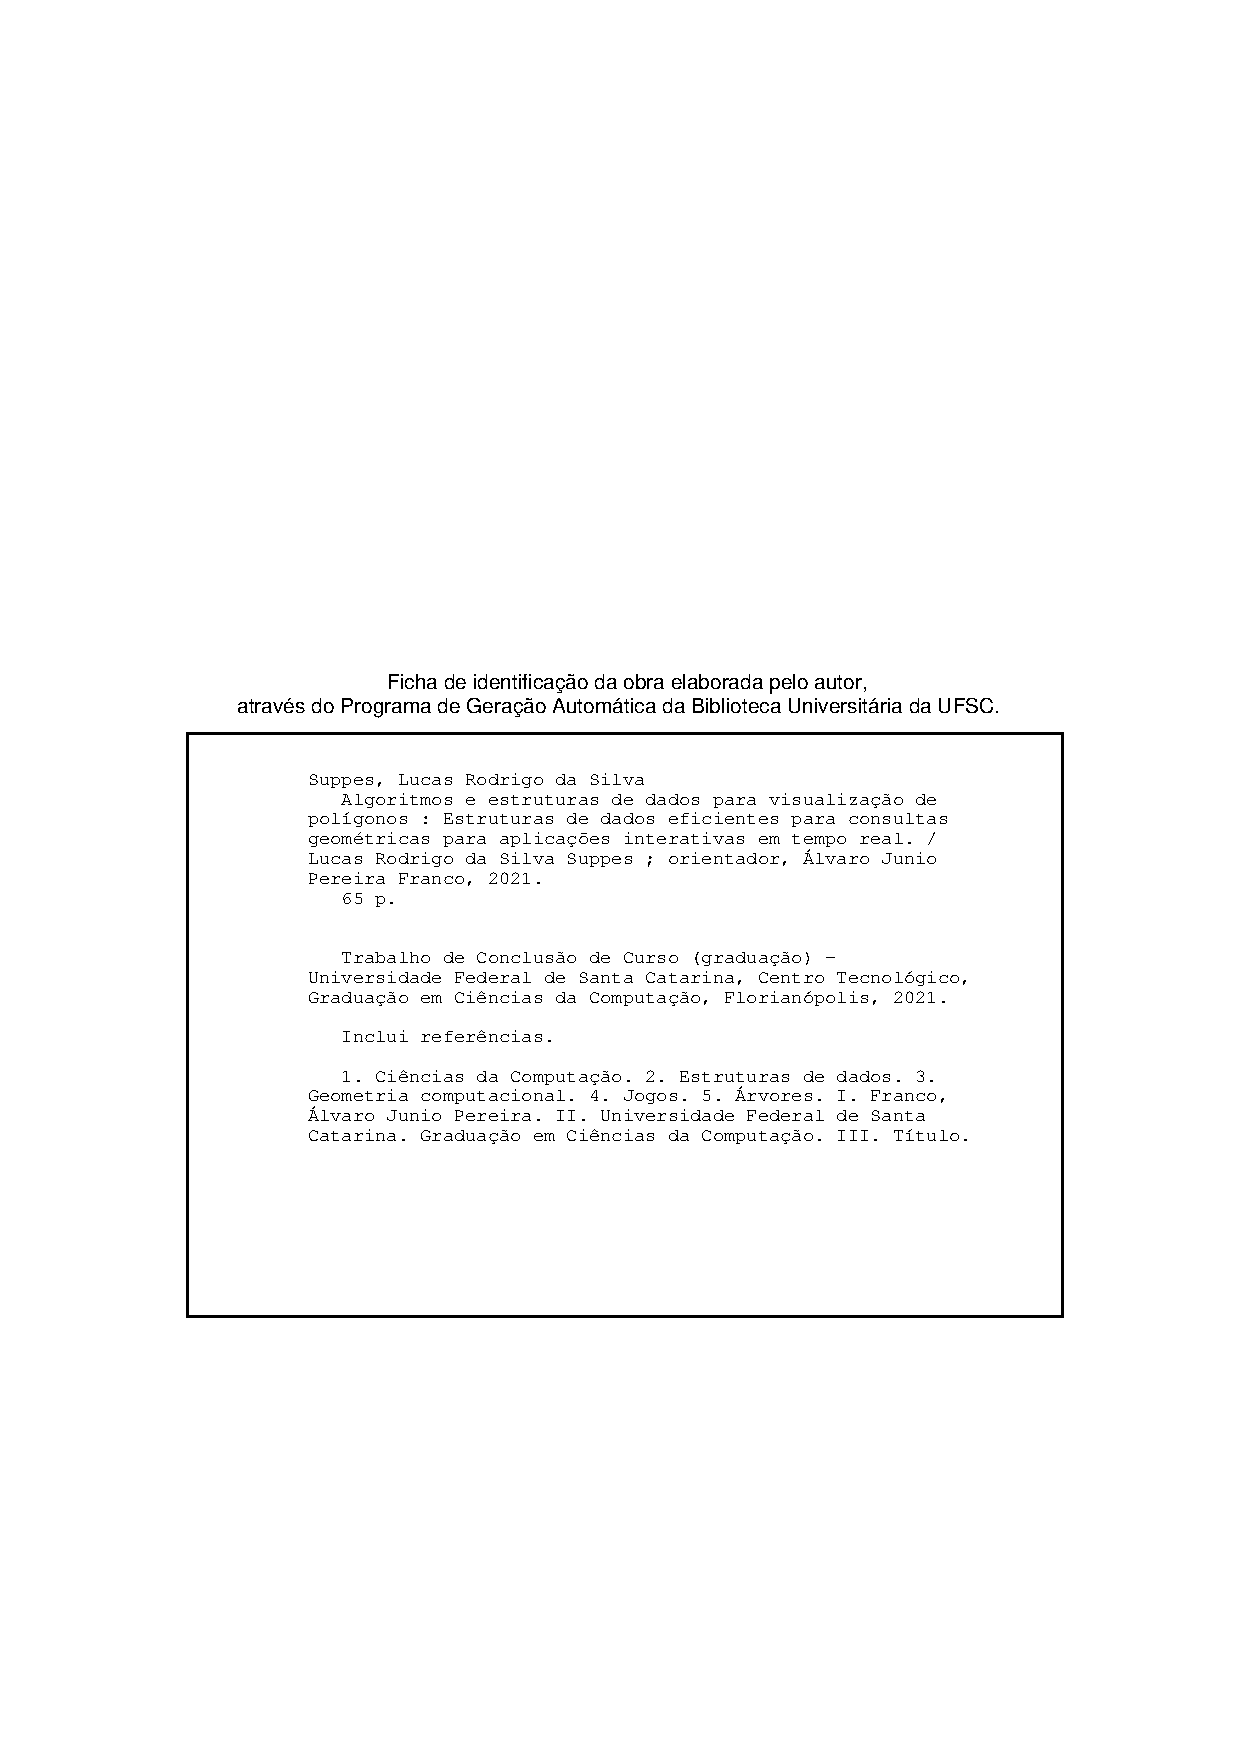
\includepdf{beforetext/Ficha_Catalografica.pdf}
\end{fichacatalografica}
% ---

% ---
% Inserir folha de aprovação
% ---

% Isto é um exemplo de Folha de aprovação, elemento obrigatório da NBR
% 14724/2011 (seção 4.2.1.3). Você pode utilizar este modelo até a aprovação
% do trabalho. Após isso, substitua todo o conteúdo deste arquivo por uma
% imagem da página assinada pela banca com o comando abaixo:
%
% \includepdf{folhadeaprovacao_final.pdf}
%
\begin{folhadeaprovacao}

  \begin{center}
    {\ABNTEXchapterfont\large\imprimirautor}

    \vspace*{\fill}\vspace*{\fill}
    \begin{center}
      \ABNTEXchapterfont\bfseries\Large\imprimirtitulo
    \end{center}
    \vspace*{\fill}
    
    \hspace{.45\textwidth}
    \begin{minipage}{.5\textwidth}
        \imprimirpreambulo
    \end{minipage}%
    \vspace*{\fill}
   \end{center}
        
   %Trabalho aprovado. \imprimirlocal, 22 de abril de 2021:
   Trabalho submetido à banca. Florianópolis, 16 de abril de 2021:

   \assinatura{\textbf{\imprimirorientador} \\ Orientador} 

   %\assinatura{\textbf{Professor} \\ Convidado 3}
   %\assinatura{\textbf{Professor} \\ Convidado 4}
      
   \begin{center}
    \vspace*{0.5cm}
    {\large\imprimirlocal}
    \par
    {\large\imprimirdata}
    \vspace*{1cm}
  \end{center}
  
\end{folhadeaprovacao}
% ---

% ---
% Dedicatória
% ---
\begin{dedicatoria}
   \vspace*{\fill}
   \centering
   \noindent
   \textit{ Este trabalho é dedicado às crianças adultas que,\\
   quando pequenas, sonharam em se tornar cientistas.} \vspace*{\fill}
\end{dedicatoria}
% ---


\begin{agradecimentos}
% Os agradecimentos principais são direcionados à Gerald Weber, Miguel Frasson,
% Leslie H. Watter, Bruno Parente Lima, Flávio de Vasconcellos Corrêa, Otavio Real
% Salvador, Renato Machnievscz\footnote{Os nomes dos integrantes do primeiro
% projeto abn\TeX\ foram extraídos de
% \url{http://codigolivre.org.br/projects/abntex/}} e todos aqueles que
% contribuíram para que a produção de trabalhos acadêmicos conforme
% as normas ABNT com \LaTeX\ fosse possível.

% Agradecimentos especiais são direcionados ao Centro de Pesquisa em Arquitetura
% da Informação\footnote{\url{http://www.cpai.unb.br/}} da Universidade de
% Brasília (CPAI), ao grupo de usuários
% \emph{latex-br}\footnote{\url{http://groups.google.com/group/latex-br}} e aos
% novos voluntários do grupo
% \emph{\abnTeX}\footnote{\url{http://groups.google.com/group/abntex2} e
% \url{http://abntex2.googlecode.com/}}~que contribuíram e que ainda
% contribuirão para a evolução do \abnTeX.
À minha mãe Cleonice que em nenhum momento teve duvidas de minha capacidade e sempre incentivou que eu trilhasse meu rumo qualquer que fosse a direção. Sempre confiou na minha bússola e compasso moral que me guiaram até onde me encontro.

À meu pai Bernardino que sem seu sopro e força jamais teria ido longe. \textit{`` Vós sois os arcos dos quais vossos filhos são arremessados como flechas vivas.'' - Khalil Gibran}

Ao meu orientador Álvaro por esse ano de trabalho incessante e seu grande carinho e suporte para que eu conseguisse executar esta obra.

À cada amigo e colega que conheci durante essa jornada. Dos que ficaram e dos que se foram. Cada letra deste trabalho tem um pouco de cada um.

À cada professor e profissional desta universidade que me passou um pouco de seu conhecimento, e em especial, à aqueles poucos professores que conseguiram  de forma especial cativar minha curiosidade para esta sublime ciência.

À flor que sem ela este trabalho jamais teria vindo a fruição. Por sempre ter acreditado em mim mesmo quando nem eu mesmo acreditava; por cada sorriso mesmo quando eu era só lagrimas; por ter sido meu alicerce quando eu era fraco.

À Ele que dá-me forças, guia-me, protege-me e orienta-me sempre.

\end{agradecimentos}


% ---
% Epígrafe
% ---
\begin{epigrafe}
    \vspace*{\fill}
    \begin{flushright}
		\textit{``Um processo computacional é de fato muito parecido como a ideia de um espirito para os magos. Não pode ser visto ou tocado. Não é composto de matéria. Entretanto, é real. Pode realizar trabalho intelectual. Pode responder questões. Pode afetar o mundo entregando dinheiro em um caixa de banco ou controlando um braço robótico em uma fábrica. Nós conjuramos programas como os magos conjuram suas magias. Eles são cuidadosamente compostos de expressões simbólicas em linguagens de programação arcanas e esotéricas que descrevem o intento para os processos executarem .'' \\
		(Structure and Interpretation of Computer Programs, pagina 2)}
	\end{flushright}
	\begin{flushright}
		\textit{``Ainda que eu andasse pelo vale da sombra da morte, \\
		não temeria mal algum, porque tu estás comigo;\\
		a tua vara e o teu cajado me consolam.\\
		(Bíblia Sagrada, Salmos 23:4)}
	\end{flushright}
\end{epigrafe}
% ---

%
% ---
% RESUMOS
% ---

% resumo em português
\setlength{\absparsep}{18pt} % ajusta o espaçamento dos parágrafos do resumo
\begin{resumo}
	\SingleSpacing
	Este trabalho apresenta um estudo de algumas estruturas de dados e técnicas para processamento de janelas. Estudamos maneiras de estruturar objetos geométricos de tal forma que consultas em janelas são respondidas eficientemente. As estruturas de dados que estudamos foram Árvore $KD$, Árvore de Alcance, Árvore de Intervalos e Árvore de Segmentos. Este trabalho utilizou todas as estruturas de dados no plano. As estruturas de dados e algoritmos de construção e consulta foram implementados. Por fim, utilizamos nossas implementações em uma aplicação que processa pontos e segmentos no plano. 
	%Tendo em mente o constante crescimento de polígonos dos objetos a serem processados, há uma necessidade de que os objetos sejam acessados de forma rápida e eficiente.

	\textbf{Palavras-chave}: Estruturas de Dados. Árvores. Geometria Computacional.
\end{resumo}

% resumo em inglês
\begin{resumo}[Abstract]
	\SingleSpacing
	\begin{otherlanguage*}{english}
		This work presents a study of some data structures and techniques to process windows. We study ways to structure geometric objects in such a way that queries in windows are quickly answered. The data structures that we study were $KD$ Tree, Range Tree, Interval Tree and Segment Tree. This work used all the data structures on the plan. The data structures and the algorithms of construction and query were implemented. Finally, we used our implementation in an application that processes points and segments on the plan.  %A study of the most common tecniques for optimizing rendering on windows.
		%Beign awere of the constant growth of the polygon count and the size of graphical applications, and the necessity for easy and quick access to the objects.

		\textbf{Keywords}: Data Structures. Trees. Computational Geometry.
	\end{otherlanguage*}
\end{resumo}



% ---
% inserir lista de ilustrações
% ---
\pdfbookmark[0]{\listfigurename}{lof}
\listoffigures*
\cleardoublepage
% ---

% ---
% inserir lista de tabelas
% ---
\pdfbookmark[0]{\listtablename}{lot}
\listoftables*
\cleardoublepage
% ---

% ---
% inserir lista de abreviaturas e siglas
% ---
%\begin{siglas}
%  \item[ABNT] Associação Brasileira de Normas Técnicas
%  \item[abnTeX] ABsurdas Normas para TeX
%\end{siglas}
% ---

% ---
% inserir lista de símbolos
% ---
%\begin{simbolos}
%  \item[$ \Gamma $] Letra grega Gama
%  \item[$ \Lambda $] Lambda
%  \item[$ \zeta $] Letra grega minúscula zeta
%  \item[$ \in $] Pertence
%\end{simbolos}
% ---

% ---
% inserir o sumario
% ---
\pdfbookmark[0]{\contentsname}{toc}
\tableofcontents*
\cleardoublepage
% ---



% ----------------------------------------------------------
% ELEMENTOS TEXTUAIS
% ----------------------------------------------------------
\textual
% ---
% 1 - Introdução
% ---
% ----------------------------------------------------------
% PARTE
% ----------------------------------------------------------
\part{Preparação da pesquisa}
% ----------------------------------------------------------
% ----------------------------------------------------------
\chapter{Introdução}
% ----------------------------------------------------------

% A contagem de polígonos em artefatos gráficos em filmes, jogos, pesquisas medicas e cientificas seguem em crescimento
% vertiginosa e apesar do Hardware acompanhar este crescimento, existem claras restrições com relação a V-RAM e a
% RAM. Com essas restrições em mente, são necessárias estruturas de dados que permitam o acesso rápido dessas
% figuras, consultas e armazenamento.
% A seleção e determinação de faces visíveis VSD.
TO-DO

% \nocite{NBR6023:2002}
% \nocite{NBR6027:2012}
% \nocite{NBR6028:2003}
% \nocite{NBR10520:2002}

% ----------------------------------------------------------
\section{Objetivos}
% ----------------------------------------------------------

O objetivo deste trabalho é estudar e implementar algoritmos e estruturas de dados que podem ser aplicadas em processamentos de objetos geométricos. Os objetos geométricos de interesse são pontos e segmentos de reta, sempre no plano. Como aplicação, podemos citar o seguinte cenário. Suponha um mundo de um jogo onde existem muitos (milhões) de objetos geométricos. O jogador enxerga alguns objetos deste mundo, isto é, os objetos que estão na câmera do jogo. Com isso, podemos aplicar as ferramentas estudadas neste trabalho para recuperar os objetos geométricos do mundo que são visíveis pela câmera.
%processamento de dados em tempo real podem se beneficiar das técnicas que descreveremos. Quando a câmera da aplicação precisa saber quais figuras geométricas precisam ser desenhadas tendo apenas a informação da posição da câmera e das coordenadas do mundo, este artigo visa o estudo de algoritmos e estruturas de dados para a solução deste tipo de problema.

% % ----------------------------------------------------------
% \subsection{Objetivo Geral}
% % ----------------------------------------------------------

% Descrição...

% % ----------------------------------------------------------
% \subsection{Objetivos Específicos}
% % ----------------------------------------------------------

% Descrição...

% % ----------------------------------------------------------
% % Introdução (exemplo de capítulo sem numeração, mas presente no Sumário)
% % ----------------------------------------------------------
% \chapter*[Introdução]{Introdução}
% \addcontentsline{toc}{chapter}{Introdução}
% % ----------------------------------------------------------

% Este documento e seu código-fonte são exemplos de referência de uso da classe
% \textsf{abntex2} e do pacote \textsf{abntex2cite}. O documento 
% exemplifica a elaboração de trabalho acadêmico (tese, dissertação e outros do
% gênero) produzido conforme a ABNT NBR 14724:2011 \emph{Informação e documentação
% - Trabalhos acadêmicos - Apresentação}.

% A expressão ``Modelo Canônico'' é utilizada para indicar que \abnTeX\ não é
% modelo específico de nenhuma universidade ou instituição, mas que implementa tão
% somente os requisitos das normas da ABNT. Uma lista completa das normas
% observadas pelo \abnTeX\ é apresentada em \citeonline{abntex2classe}.

% Sinta-se convidado a participar do projeto \abnTeX! Acesse o site do projeto em
% \url{http://abntex2.googlecode.com/}. Também fique livre para conhecer,
% estudar, alterar e redistribuir o trabalho do \abnTeX, desde que os arquivos
% modificados tenham seus nomes alterados e que os créditos sejam dados aos
% autores originais, nos termos da ``The \LaTeX\ Project Public
% License''\footnote{\url{http://www.latex-project.org/lppl.txt}}.

% Encorajamos que sejam realizadas customizações específicas deste exemplo para
% universidades e outras instituições --- como capas, folha de aprovação, etc.
% Porém, recomendamos que ao invés de se alterar diretamente os arquivos do
% \abnTeX, distribua-se arquivos com as respectivas customizações.
% Isso permite que futuras versões do \abnTeX~não se tornem automaticamente
% incompatíveis com as customizações promovidas. Consulte
% \citeonline{abntex2-wiki-como-customizar} par mais informações.

% Este documento deve ser utilizado como complemento dos manuais do \abnTeX\ 
% \cite{abntex2classe,abntex2cite,abntex2cite-alf} e da classe \textsf{memoir}
% \cite{memoir}. 

% Esperamos, sinceramente, que o \abnTeX\ aprimore a qualidade do trabalho que
% você produzirá, de modo que o principal esforço seja concentrado no principal:
% na contribuição científica.

% Equipe \abnTeX 

% Lauro César Araujo


% ---

\lipsum[1]
% ---
% 2 - Capítulo 2
% ---

% ----------------------------------------------------------
% PARTE
% ----------------------------------------------------------
\part{Referenciais teóricos}
% ----------------------------------------------------------
% ----------------------------------------------------------
\chapter{Estruturas de busca de pontos}\label{cap:desenvolvimento}
% ----------------------------------------------------------
Neste capitulo apresenta-se uma visão de como funcionam os algoritmos e estruturas de dados base para o desenvolvimento
de algoritmos para renderização em janela acesso rápido para estruturas geométricas.
Sao os algoritmos e estruturas de dados base para a construção de um controle de janela para acesso rapido de poligonos
em janela.



% ----------------------------------------------------------
\section{Arvores KD}
% ----------------------------------------------------------

Uma Arvore KD é uma arvore binaria onde cada folha é um ponto \textit{k-dimensional}.
E cada nodo não-folha é um corte do espaço, representando implicitamente um hiperplano.
Pontos a esquerda desse hiperplano estão na subárvore da esquerda, e respectivamente para o lado direito.
Cada nodo é associado com uma das \textit{k dimensões}. Então, a citar um exemplo, se dado nodo divide o eixo
x, a subárvore a esquerda contem os pontos com o eixo x menor que o ponto de corte.

\begin{figure}[htb]
    \caption{\label{fig:Fig_1}Arvore k\textit{dimensional} - 3D}
    \begin{center}
        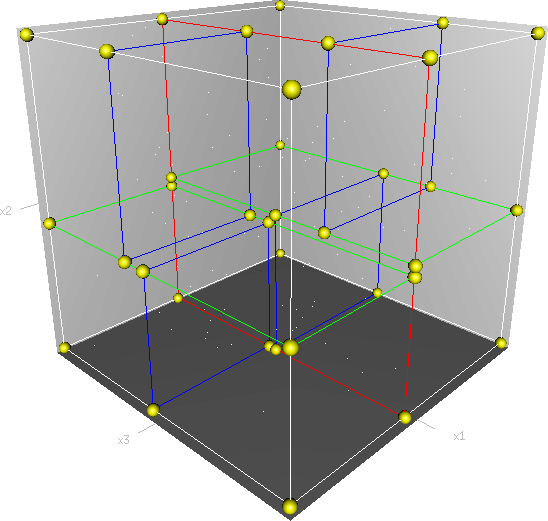
\includegraphics[width=\linewidth/2]{./images/3dtree.png}
    \end{center}
    \fonte{GPL}
\end{figure}

\subsection{Construção da Árvore}
A termos didáticos segue a construção da arvore KD de 2 dimensões.
Seja \textit{P} o conjunto de \textit{n} pontos em um plano.

Uma busca de alcance 2-dimensional em \textit{P} é uma busca de quais pontos da busca estão
entre o retângulo de busca \([x,x']  \times  [y,y']\). Um ponto \(p:= (p_x, p_y)\) está dentro do retângulo
de busca se e somente se:

\[
p_x \in [x, x'] \textrm{ e } p_y \in [y, y`]
\]

Podemos dizer que uma busca 2-dimensional é composta de duas sub-buscas 1-dimensional, uma no
eixo \(x\)-coordenada de um dos pontos e um na \(y\)-coordenada.

\begin{figure}[htb]
    \caption{\label{fig:Fig_2}Busca em alcance \textit{dimensional} - 2D}
    \begin{center}
        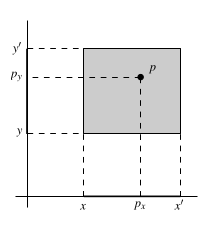
\includegraphics{images/search_range.png}
    \end{center}
    \fonte{Computational Geometry}
\end{figure}

Na construção de uma arvore para 2 dimensões, cada ponto tem uma \(x\)-coordenada e uma
\(y\)-coordenada.
Seguimos então escolhendo um eixo inicial e salvando o valor de corte deste eixo que divide
os pontos deste eixo em dois conjuntos, e no próximo nível da arvore, alterna-se o eixo e repete-se
o processo recursivamente.


\begin{figure}[htb]
    \caption{\label{fig:Fig_3} Arvore 2D}
    \begin{center}
        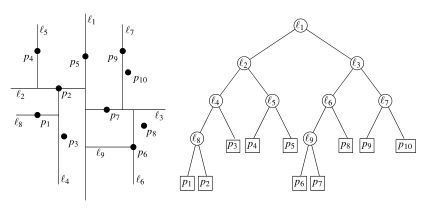
\includegraphics{images/kd_tree1.png}
    \end{center}
\end{figure}

Na raiz ordena-se todos os pontos e divide o conjunto de pontos \(P\) com uma linha vertical
\(l\) que divide os pontos pelo eixo \(x\). Guarda-se o valor de \(x_v\) no nodo e alterna-se o
eixo.
Agora, recursivamente repete o processo para os dois subconjuntos de pontos:
Ordena-se os pontos pelo eixo \(y\) e divide o conjunto e encontra-se a reta horizontal que
subdivide os pontos e guarda no nodo do valor de corte \(y\).
A condição de parada é até quando o conjunto de pontos restantes contiver apenas um ponto.
Este sendo então o nodo folha.


\begin{algorithm}\caption{The Bellman-Kalaba algorithm}\begin{algorithmic}[1]\Procedure {BellmanKalaba}{$G$, $u$, $l$, $p$}\ForAll {$v \in V(G)$}\State $l(v) \leftarrow \infty$\EndFor\State $l(u) \leftarrow 0$\Repeat\For {$i \leftarrow 1, n$}\State $min \leftarrow l(v_i)$\For {$j \leftarrow 1, n$}\If {$min > e(v_i, v_j) + l(v_j)$}\State $min \leftarrow e(v_i, v_j) + l(v_j)$\State $p(i) \leftarrow v_j$\EndIf\EndFor\State $l’(i) \leftarrow min$\EndFor\State $changed \leftarrow l \not= l’$\State $l \leftarrow l’$\Until{$\neg changed$}\EndProcedure\Statex\Procedure {FindPathBK}{$v$, $u$, $p$}\If {$v = u$}\State \textbf{Write} $v$\Else\State $w \leftarrow v$\While {$w \not= u$}\State \textbf{Write} $w$\State $w \leftarrow p(w)$\EndWhile\EndIf\EndProcedure\end{algorithmic}\end{algorithm}
% \begin{algorithm}
%     \caption{ConstroiArvoreKD($Pontos, profundidade$)}
%     \begin{algorithmic}
%         \IF{P contem apenas um ponto}
%         \RETURN $P$
%         \ELSE
%         \STATE{
%             \IF{$profundidade$ é par}
%             \STATE{
%                 Divide P em dois subconjuntos com um linha vertical $l$ pela mediana da $x-coordenada$
%                 dos pontos em P. Seja $P_1$ o conjunto dos pontos à esquerda de $l$ e seja
%                 $P_2$ o conjunto de pontos à direita de $l$.
%             }
%             \ELSE
%             \STATE{
%                 Divide P em dois subconjuntos com um linha horizontal $l$ pela mediana da $y-coordenada$
%                 dos pontos em P. Seja $P_1$ o conjunto dos pontos acima de $l$ e seja
%                 $P_2$ o conjunto de pontos à abaixo de $l$.
%             }
%             \ENDIF
%         }
%         \ENDIF

%         \STATE $v_{esquerda} \leftarrow $ ConstroiArvoreKD($P_1, profundidade+1$)
%         \STATE $v_{direita} \leftarrow $ ConstroiArvoreKD($P_2, profundidade+1$)
%         Cria um nodo $v$ guardando $l$ e fazendo $v_esquerda$ o nodo da esquerda
%         de $v$ e fazendo $v_direita$ nodo da direita de $v$.

%         \RETURN $v$
%     \end{algorithmic}
% \end{algorithm}

\subsection{Busca com alcance}

Agora retomamos para o algoritmo de busca. Podemos imaginar que os pontos na subárvore à esquerda
da raiz, estão limitados à direita pela reta com o eixo \(x\) com valor de \(x \leq l_1\).
Enquanto os pontos na subárvore à direita do nodo \(l_1\) estão limitados com o eixo \(x > l_1\).

A exemplo: o nodo \(l_4\), a região correspondente de \(l_4\) é limitada à esquerda de
\(l_1\) e abaixo de \(y\) do nodo \(l_2\).

\begin{figure}[htb]
    \caption{\label{fig:Fig_4} Área respectiva de um nodo}
    \begin{center}
        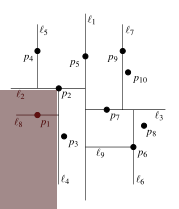
\includegraphics{images/kd_tree2.png}
    \end{center}
\end{figure}

Denotaremos esta área de um nodo \(v\) como \(regiao(v)\). A região da raiz é simplesmente
(no caso de uma arvore 2D) o plano inteiro.
Portanto o algoritmo buscará a subárvore de \(v\) somente se o retângulo de busca intersectar
a \(regiao(v)\).
O algoritmo de busca funciona descendo a arvore mas visitando somente os nodos que a
\(regiao(v)\) intersecta o retângulo da busca. Quando uma \(regiao(v)\) esta contido no
retângulo de busca retornamos todos os pontos na subárvore.
Quando chegarmos nos nodos folhas temos de checar se o nodo esta dentro da busca, se tiver,
retorna-o.

Segue o algoritmo que recebe como parâmetros a raiz da arvore-KD e o retângulo de busca \(R\).
Usa-se uma chamada \(RetornaSubarvore(v)\) que atravessa a arvore de nodo \(v\) e retorna
todos os pontos nas suas folhas. Segue como notação \(fe(v)\) sendo o filho da esquerda e
\(fd(v)\) o filho da direita do nodo \(v\).


% \begin{algorithm}
%     \caption{BuscaEmArvoreKD($v, Busca$)}
%     \begin{algorithmic}
%         \IF{v é folha}
%         \STATE{Retorna o ponto de $v$ se estiver dentro da $Busca$}
%         \ELSE
%         \STATE{
%             \IF{$regiao(fe(v))$ está contido na $Busca$}
%             \STATE{$RetornaSubarvore(v)$}
%             \ELSE
%             \STATE{
%                 \IF{$regiao(fe(v))$ intersecta $Busca$}
%                 \STATE{
%                     $BuscaEmArvoreKD(fe(v), Busca)$
%                 }
%                 \ENDIF
%             }
%             \ENDIF

%             \IF{$regiao(fd(v))$ está contido na $Busca$}
%             \STATE{$RetornaSubarvore(v)$}
%             \ELSE
%             \STATE{
%                 \IF{$regiao(fd(v))$ intersecta $Busca$}
%                 \STATE{
%                     $BuscaEmArvoreKD(fd(v), Busca)$
%                 }
%                 \ENDIF
%             }
%             \ENDIF
%         }
%         \ENDIF
%     \end{algorithmic}
% \end{algorithm}

A principal comparação realizada é checar se a área de \(Busca\) intersecta a região
de um nodo \(v\). Para isso precisamos computar \(regiao(v)\) para todos os nodos \(v\)
durante a fase de construção da arvore.
Uma alternativa é manter a região salva nas chamadas recursivas usando as linhas guardadas
nos nodos internos. Por exemplo a região correspondente ao filho esquerda de um nodo
\(v\) em uma profundidade par (no exemplo 2D, analisamos no eixo \(x\)) pode ser calculado com:
\[
    regiao(fe(v)) = regiao(v) \cap l(v)^{esquerda}
\],
onde \(l(v)\) é a linha que divide o eixo salvo em \(v\), e \(l(v)^{esquerda}\) é a metade
esquerda do plano.


% ----------------------------------------------------------
\section{Arvore de Intervalos}
% ----------------------------------------------------------

% No que diz respeito à estrutura do trabalho, recomenda-se que:
% \begin{alineas}
% 	\item o texto deve ser justificado, digitado em cor preta, podendo utilizar outras cores somente para as ilustrações;
% 	\item utilizar papel branco ou reciclado para impressão;
% 	\item os elementos pré-textuais devem iniciar no anverso da folha, com exceção da ficha catalográfica ou ficha de identificação da obra;
% 	\item os elementos textuais e pós-textuais devem ser digitados no anverso e verso das folhas, quando o trabalho for impresso. As seções primárias devem começar sempre em páginas ímpares, quando o trabalho for impresso. Deixar um espaço entre o título da seção/subseção e o texto e entre o texto e o título da subseção.
% \end{alineas}

% No \autoref{qua:Quadro_1} estão as especificações para a formatação do texto.

% \begin{quadro}[htb]
% 	\centering
% 	\caption{\label{qua:Quadro_1}Formatação do texto.}
% 	\begin{tabular}{|l|p{11cm}|}
% 		\hline
% 		\textbf{Formato do papel} & A4.                                                                                                                                                                                                                                                                                                                                                                                                                                 \\ \hline
% 		\textbf{Impressão}        & A norma recomenda que caso seja necessário imprimir, deve-se utilizar a frente e o verso da página.                                                                                                                                                                                                                                                                                                                                 \\ \hline
% 		\textbf{Margens}          & Superior: 3, Inferior: 2, Interna: 3 e Externa: 2. Usar margens espelhadas quando o  trabalho for impresso.                                                                                                                                                                                                                                                                                                                         \\ \hline
% 		\textbf{Paginação}        & As páginas dos elementos pré-textuais devem ser contadas, mas não numeradas. Para trabalhos digitados somente no anverso, a numeração das páginas deve constar no canto superior direito da página, a 2 cm da borda, figurando a partir da primeira folha da  parte textual. Para trabalhos digitados no anverso e no verso, a numeração deve constar no canto superior direito, no anverso, e no canto superior esquerdo no verso. \\ \hline
% 		\textbf{Espaçamento}      & O texto deve ser redigido com espaçamento entre linhas 1,5, excetuando-se as citações de mais de três linhas, notas de rodapé, referências, legendas das ilustrações e das tabelas, natureza (tipo do trabalho, objetivo, nome da instituição a que é submetido e área de concentração), que devem ser digitados em espaço simples, com fonte menor. As referências devem ser separadas entre si por um espaço simples em branco.   \\ \hline
% 		\textbf{Paginação}        & A contagem inicia na folha de rosto, mas se insere o número da página na introdução até o final do trabalho.                                                                                                                                                                                                                                                                                                                        \\ \hline
% 		\textbf{Fontes sugeridas} & Arial ou Times New Roman.                                                                                                                                                                                                                                                                                                                                                                                                           \\ \hline
% 		\textbf{Tamanho da fonte} & \textbf{Fonte tamanho 12 para o texto}, incluindo os títulos das seções e subseções. As citações com mais de três linhas, notas de rodapé, paginação, dados internacionais de catalogação, legendas e fontes das ilustrações e das tabelas devem ser de tamanho menor. Adotamos, neste \textit{template} \textbf{fonte tamanho 10}.                                                                                                 \\ \hline
% 		\textbf{Nota de rodapé}   & Devem ser digitadas dentro da margem, ficando separadas por um espaço simples por entre as linhas e por filete de 5 cm a partir da margem esquerda. A partir da segunda linha, devem ser alinhadas embaixo da primeira letra da primeira palavra da primeira linha.                                                                                                                                                                 \\ \hline
% 	\end{tabular}
% 	\fonte{\textcite{NBR14724:2011}.}
% \end{quadro}

% % ----------------------------------------------------------
% \subsubsection{As ilustrações}
% % ----------------------------------------------------------

% Independentemente do tipo de ilustração (quadro, desenho, figura, fotografia, mapa, entre outros), a sua identificação aparece na parte superior, precedida da palavra designativa.

% \begin{citacao}
% 	Após a ilustração, na parte inferior, indicar a fonte consultada (elemento obrigatório, mesmo que seja produção do próprio autor), legenda, notas e outras informações necessárias à sua compreensão (se houver). A ilustração deve ser citada no texto e inserida o mais próximo possível do texto a que se refere. \cite[p. 11]{NBR14724:2011}.
% \end{citacao}

% % ----------------------------------------------------------
% \subsubsection{Equações e fórmulas}
% % ----------------------------------------------------------

% As equações e fórmulas devem ser destacadas no texto para facilitar a leitura.  Para numerá-las, usar algarismos arábicos entre parênteses e alinhados à direita. Pode-se adotar uma entrelinha maior do que a usada no texto \cite{NBR14724:2011}.

% Exemplos, \autoref{eq:Eq_1} e \autoref{eq:Eq_2}.

% \begin{equation}\label{eq:Eq_1}
% 	\gls{C} = 2 \gls{pi} \gls{r}
% \end{equation}

% \begin{equation}\label{eq:Eq_2}
% 	\gls{A} = \gls{pi} \gls{r}^2
% \end{equation}
% ----------------------------------------------------------
\section{Arvore de Segmentos}
% ----------------------------------------------------------

% De acordo com \textcite{ibge1993}, tabela é uma forma não discursiva de apresentar informações em que os números representam a informação central. Ver \autoref{tab:Tab_1}.

% \begin{table}[htb]
% 	\ABNTEXfontereduzida
% 	\caption{\label{tab:Tab_1}Médias concentrações urbanas 2010-2011.}
% 	\begin{tabular}{@{}p{3.0cm}p{1.5cm}p{2cm}p{2.5cm}p{2.5cm}p{2.5cm}@{}}
% 		\toprule
% 		\textbf{Média concentração urbana} & \multicolumn{2}{l}{\textbf{População}} & \textbf{Produto Interno Bruto – PIB (bilhões R\$)} & \textbf{Número de empresas} & \textbf{Número de unidades locais}         \\ \midrule
% 		\textbf{Nome}                      & \textbf{Total}                         & \textbf{No Brasil}                                 &                             &                                    &       \\
% 		Ji-Paraná (RO)                     & 116 610                                & 116 610                                            & 1,686                       & 2 734                              & 3 082 \\
% 		Parintins (AM)                     & 102 033                                & 102 033                                            & 0,675                       & 634                                & 683   \\
% 		Boa Vista (RR)                     & 298 215                                & 298 215                                            & 4,823                       & 4 852                              & 5 187 \\
% 		Bragança (PA)                      & 113 227                                & 113 227                                            & 0,452                       & 654                                & 686   \\ \bottomrule
% 	\end{tabular}
% 	\fonte{\textcite{ibge2016}.}
% \end{table}
% ---

% ---
% 3 - Capítulo 3
% ---
% ----------------------------------------------------------
\chapter{Seção}
% ----------------------------------------------------------

Este \textit{template} contém algumas seções criadas na tentativa de facilitar seu uso. No entanto, não há um limite máximo ou mínimo de seção a ser utilizado no trabalho. Cabe a cada autor definir a quantidade que melhor atenda à sua 
necessidade.  
% ---

\lipsum[2-3]

% ---
% 4 - Conclusão
% ---
%\phantompart

% ----------------------------------------------------------
% PARTE
% ----------------------------------------------------------
\part{Resultados}
% ----------------------------------------------------------
% ----------------------------------------------------------
\chapter{Resultados}
% ----------------------------------------------------------
Neste capitulo falaremos das nossas implementações e de nossos resultados com algumas delas. As estruturas\footnote{Afim de a aplicação ser agnóstica de sistema, utilizamos o programa pipenv que permite criar ambientes Python com as dependencias necessárias. Instruções de uso estão disponíveis no arquivo README do projeto. \url{https://github.com/lrdass/theia}} foram implementadas na linguagem Python, e para validação visual preferimos imagens SVG por serem fáceis de interpretar e de gerar imagens teste. Além da implementação das estruturas desenvolvemos dois casos de testes para validar as estruturas. O primeiro é uma aplicação onde há um mapa com movimento livre com inúmeros pontos. A ideia deste programa era validar tanto a aplicação para jogos 2D quanto 3D. Para um jogo 2D, poderíamos substituir cada ponto por texturas do jogo, e teríamos um mapa virtualmente infinito em dimensões. Validamos para 3D, pois, para estender a estrutura utilizada para 3D é trivial, e portanto, buscamos neste capitulo validar que podemos consultar no plano grandes ordens de grandeza de pontos sem grandes impactos na performance. Validamos esta ideia mostrando os tempos de consulta para grandes valores de pontos. O segundo programa é um mapa do brasil com grande resolução de segmentos e movimento de câmera livre por este mapa. Validamos a aplicação mostrando que seria inviável ter uma aplicação de tempo real sem as estruturas utilizadas. Construímos cada uma das estruturas de dados apresentadas no texto e cada uma delas tem métodos auxiliares para construir figura SVG com pontos aleatórios com janelas aleatórias, e a construção da árvore em cima do arranjo de pontos desta imagem e a saída do programa como outra figura SVG com os pontos dentro da janela indicados com a cor verde.Todas as estruturas foram construídas visando apenas a consulta em janela. Portanto como demonstrado no texto nos atentamos apenas aos métodos de construção e consulta. As estruturas de consulta para segmentos por sua vez foram construídas, como visto no trabalho até aqui, para consultas das bordas e portanto trabalham em conjunto com as estruturas de consultas de pontos. Para interpretarmos as imagens utilizamos a biblioteca \textit{xml} e interpretamos as figuras SVG como XML.Usamos a mesma biblioteca tanto para a leitura quanto escrita das figuras após a consulta. 

\section{Aplicação árvore de intervalos}\label{cap:application-points}
Em uma aplicação tridimensional poderíamos construir cenas arbitrariamente grandes de tal forma que organizaríamos os objetos da cena $3D$ com uma árvore de alcance de 3 dimensões. Consultaríamos nesta árvore, portanto, o cubo representado pela câmera. Reportando somente quais estruturas estão dentro da janela e então enviaríamos para o pipeline gráfico \ref{cap:cg} para desenharmos na tela. Podemos pensar em uma limitação para um jogo que precisa manter todos os objetos geométricos no pipeline. O número de objetos geométricos seria limitado pela memória do pipeline. 
A partir destas constatações podemos recriar este comportamento construindo uma árvore de alcance tridimensional com todos os seus objetos, e carregamos para memória da placa de video apenas o que é retornado da consulta. Necessitando de apenas uma tela de carregamento para construir a árvore.

\begin{figure}[h!]
    \centering
    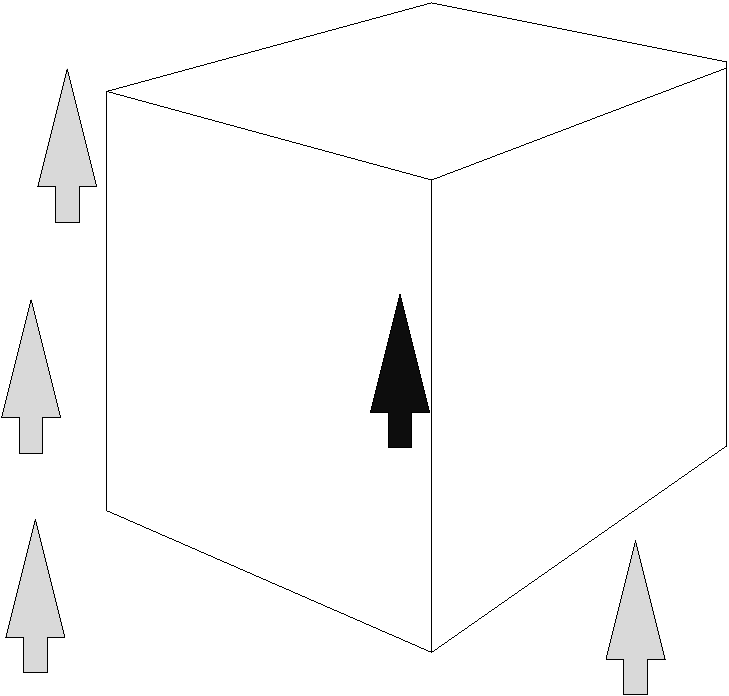
\includegraphics[scale=0.4]{images/3d-query-example.pdf}
    \caption{Exemplo de cena tridimensional com uma consulta retornando apenas os objetos dentro da janela}
    \label{fig:3d-query-example}
\end{figure}

Para justificarmos esta aplicação, construímos uma versão simplificada do problema em duas dimensões. Criamos aleatoriamente pontos no plano e construímos uma árvore de alcance bidimensional. Em cada laço de execução do programa, consultamos a árvore com a janela, e desenhamos apenas os pontos dentro da janela. A solução trivial deste problema sem as árvores de alcance é consultar cada ponto e então desenha-lo e deixar o algoritmo de recorte \cite{folley01} não desenhar na tela. Porem, ainda iteraria sobre estes para poder constatar que não estão na janela. Enquanto utilizando a árvore, temos uma maneira eficiente de consultar e desenhar apenas os pontos dentro da janela.

\begin{figure}[h!]
\centering
\begin{minipage}{.5\textwidth}
  \centering
  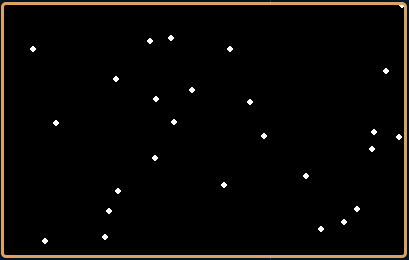
\includegraphics[width=.8\linewidth]{images/Captura de tela de 2021-04-16 11-43-23.png}
 
  \label{fig:sub1}
\end{minipage}%
\begin{minipage}{.5\textwidth}
  \centering
  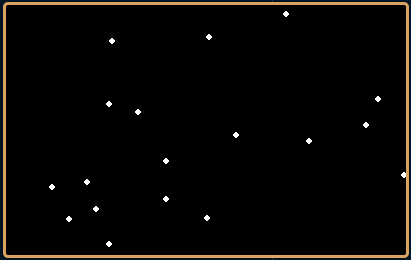
\includegraphics[width=.8\linewidth]{images/Captura de tela de 2021-04-16 11-43-35.png}
  
  \label{fig:sub2}
\end{minipage}
\caption{Aplicação construída com pontos no plano e consultas em tempo real}
\label{fig:test}
\end{figure}

Como jogos são aplicações de tempo real, temos que pensar em restrições de tempo. Jogos modernos tem objetivos de entregar entre 30 e 60 quadros por segundo. Considerando o pior caso temos $\frac{1}{30} \approx 0.0334$ segundos para computações entre cada quadro.

\begin{table}[h!]
\centering
\begin{tabular}{|c c c |} 
 \hline
 Pontos & Média do Tempo (s) & Desvio Padrão (s) \\%$\sigma$ \\
 \hline
 1000  & $0.00012955069541931$  & $1.3212002262037\times 10^{-5}$ \\
\hline
 10000  & $0.00013832251230876$  & $2.0937153306017\times 10^{-5}$ \\
\hline
 100000  & $0.00015597189626386$  & $2.8073955196226\times 10^{-5}$ \\
\hline
\end{tabular}
\caption{Tabela comparativa do número de pontos e o tempo para reportar os pontos em uma janela proporcional ao tamanho do conjunto de pontos testado}
\label{table:1}
\end{table}
\begin{table}[h!]
\centering
\begin{tabular}{|c c |} 
 \hline
 Incremento médio tempo consulta(s) para cada $10^{n} $ pontos & Desvio Padrão (s) \\%$\sigma$ \\
 \hline
 $0,00001321$  & $ 6.276986896593 \times 10^{-6}$ \\
\hline
\end{tabular}
\caption{Há um incremento médio de 13,21 microssegundos para cada $10^{n}$ pontos na consulta }
\label{table:1}
\end{table}

Com base na tabela anterior temos bastante confiança de que a estrutura de dados está dentro do tempo limite de computação para cada quadro desenhado, até mesmo aumentando o número de pontos. Mostrando que o crescimento com um fator de $10^n$ o tempo da consulta ainda permanece na casa dos $0.1$ milissegundos.

\section{Aplicação árvore de segmentos}\label{cap:application-segment}
Em aplicações de tempo real pode ser que exista apenas um objeto com grande complexidade. Programas que permitem ilustração em tempo real, por exemplo, estão mais interessados em conhecer se determinado segmento do objeto sendo desenhado está dentro da janela. Ou mapeamento tridimensional de um sistema cardiovascular em tempo real em que temos uma malha de um único objeto com grande complexidade e, para visualizá-lo, temos que carregar apenas um recorte deste objeto complexo. Em OpenGL \cite{opengl} temos um arranjo com as posições dos vértices chamado $Vertex Array$ e um segundo arranjo que contém uma ordem de cada vértice para formar os triângulos chamado $Element Array$. Podemos portanto interpretar estes dois arranjos e construir os segmentos pois sabemos que cada aresta de um triângulo é um segmento. E assim utilizar estes para construir e consultar com a árvore de segmentos. Para simplificarmos este problema tridimensional, desenvolvemos uma aplicação mostrado na Figura \ref{fig:brazil_map_app} que navega pelo mapa do Brasil com alta resolução de segmentos em tempo real. 

\begin{table}[h!]
\centering
\parbox{.5\linewidth}{
\centering
\begin{tabular}{| c c |} 
 \hline
 Média do Tempo (s) & Desvio Padrão (s) \\%$\sigma$ \\
 \hline
 $0.005857$  & $0.003753$ \\
\hline
\end{tabular}
\caption{Utilizando a estrutura de dados para consultar os segmentos}
\label{table:1}
}
\parbox{.5\linewidth}{
\centering
\begin{tabular}{| c c |} 
 \hline
 Media do Tempo (s) & Desvio Padrão (s) \\%$\sigma$ \\
 \hline
 $0.148667$  & $0.017494$ \\
\hline
\end{tabular}
\caption{Sem a estrutura de dados consultando linearmente}
\label{table:1}
}
\end{table}

A consulta linear está inviável para uma aplicação de tempo real. Imaginando a mesma restrição de 30 quadros por segundo tendo $\frac{1}{30} \approx 0.0334$ segundos para calcular um quadro seria inviável atingir o objetivo sem a árvore de segmentos. A consulta linear alcançaria no máximo $\frac{1}{0.1487} \approx 6.72$ quadros por segundo nos nossos experimentos.


\chapter*[Conclusão]{Conclusão}
\addcontentsline{toc}{chapter}{Conclusão}
% ---

\lipsum[31-33]

% ----------------------------------------------------------
% Finaliza a parte no bookmark do PDF
% para que se inicie o bookmark na raiz
% e adiciona espaço de parte no Sumário
% ----------------------------------------------------------
%\phantompart

% ---
% Conclusão (outro exemplo de capítulo sem numeração e presente no sumário)
% ---

% ----------------------------------------------------------
% ELEMENTOS PÓS-TEXTUAIS
% ----------------------------------------------------------
\postextual
% ----------------------------------------------------------
% ----------------------------------------------------------
% Referências bibliográficas
% ----------------------------------------------------------
\begingroup
\printbibliography[title=REFERÊNCIAS]
\endgroup

% ----------------------------------------------------------
% Glossário
% ----------------------------------------------------------
%
% Consulte o manual da classe abntex2 para orientações sobre o glossário.
%
%\glossary

% ----------------------------------------------------------
% Apêndices
% ----------------------------------------------------------

% ---
% Inicia os apêndices
% ---
\begin{apendicesenv}
	%	\partapendices* 
	% ----------------------------------------------------------
%\chapter{Descrição 1}
% ----------------------------------------------------------

%Textos elaborados pelo autor, a fim de completar a sua argumentação. Deve ser precedido da palavra APÊNDICE, identificada por letras maiúsculas consecutivas, travessão e pelo respectivo título. Utilizam-se letras maiúsculas dobradas quando esgotadas as letras do alfabeto. 

\end{apendicesenv}
% ---


% ----------------------------------------------------------
% Anexos
% ----------------------------------------------------------

% ---
% Inicia os anexos
% ---
\begin{anexosenv}
	%	\partanexos*
	% ----------------------------------------------------------
\chapter{Descrição 2}
% ----------------------------------------------------------

São documentos não elaborados pelo autor que servem como fundamentação (mapas, leis, estatutos). Deve ser precedido da palavra ANEXO, identificada por letras maiúsculas consecutivas, travessão e pelo respectivo título. Utilizam-se letras maiúsculas dobradas quando esgotadas as letras do alfabeto. 

\end{anexosenv}

%---------------------------------------------------------------------
% INDICE REMISSIVO
%---------------------------------------------------------------------
%\phantompart
%\printindex
%---------------------------------------------------------------------

\end{document}